% Para estilizar código
\section{Introducción}
% TODO: insertar chamu sobre sistemas similares disponibles, etc.
En el ámbito universitario resulta necesario mantener informadas a las personas sobre una amplia variedad de hechos, noticias y acontecimientos que sucedieron o sucederán, desde la ubicación de un aula hasta la notificación de la cancelación de una clase. Muchas veces estas notificaciones son sobre cuestiones muy efímeras, lo que requiere rapidez para empezar a transmitirlas y facilidad para tener el alcance necesario.

En las facultades de la Universidad Nacional de La Plata se consumen muchos recursos para cumplir este fin, a través de afiches, pancartas, panfletos, etc. los cuales, pese a ser de barata fabricación, no tienen una vida útil muy extensa. Además todas estas formas de comunicacion se basan en el uso de papel, que tras ser utilizado debe desecharse debido a la imposibilidad de reutilizarlo, generando una cantidad de residuos significativa. Si se tiene en cuenta que también generan una polución visual considerable, por la gran cantidad de estos distribuidos en todos los lugares transitables, resulta prudente considerar una nueva forma de comunicación.

% TODO: Mencionar sobre otros carteles comercialmente disponibles
Surge así la idea de desarrollar de un cartel electrónico reutilizable, capaz de ser configurado remotamente por las autoridades competentes, con el fin de proveer una forma de comunicación masiva más limpia, clara y menos dañina para el medio ambiente.

En este informe se describe todas las fases del desarrollo de un proyecto para la asignatura Taller de Proyecto 1. El proyecto consiste en el diseño y desarrollo de un sistema de cartel luminoso cuyo contenido es configurable de forma remota. El cartel tiene conectividad WiFi, con lo que es capaz de formar parte de una red IP.

El proyecto utilizó un proceso de desarrollo de cascada, como se muestra en la figura \ref{fig:waterfall}.

\begin{figure}[!ht]
	\centering
	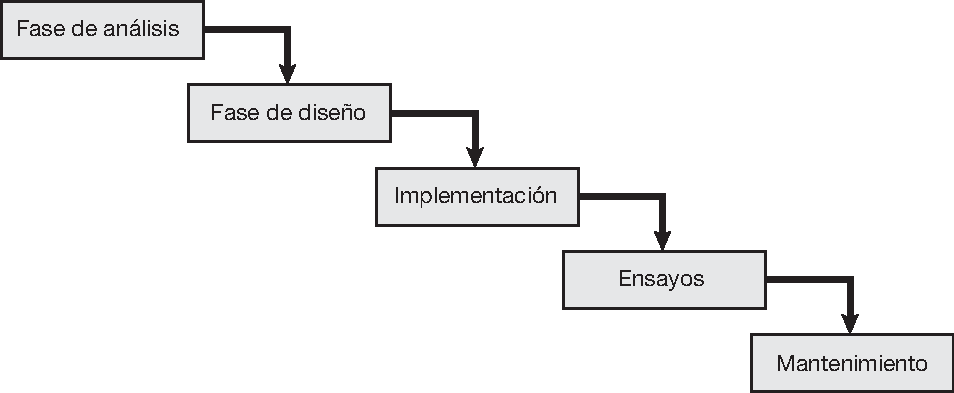
\includegraphics[width=0.8\linewidth]{imagenes/waterfall.pdf}
	\caption{Modelo en cascada de desarrollo.}
	\label{fig:waterfall}
\end{figure}

A lo largo de este informe se documentarán las fases de desarrollo previamente mencionadas.

En la sección \ref{part:analisis} se habla sobre los requerimientos y especificaciones del sistema, detallando que funcionalidades debe tener y a cuáles restricciones está sujeto.

Luego, en la sección \ref{part:diseno}, se mencionan las componentes que constituyen el sistema, se explicitan modelos que describen el comportamiento del sistema, la interfaz de usuario y la arquitectura del software. También se muestran los esquemáticos que especifican la conexión de los componentes.

En la sección de implementación se documenta como se fue dando el proceso de desarrollo de software y la implementación física del hardware.

En la sección de ensayos se documenta los resultados de las pruebas que se realizaron sobre el sistema en funcionamiento.

Por último, se anexa como apéndice una guía instructiva que explica los pasos necesarios para poner en marcha el sistema.

\section{Objetivos del proyecto}
El objetivo primario de este proyecto es el diseño implementación de un cartel luminoso que pueda ser configurado remotamente por un usuario. No se tiene como objetivo realizar un producto diseñado de manera que sea económicamente viable producirlo en masa, sino más bien el desarrollo de un prototipo a modo de prueba de concepto.

El objetivo puede ser divido en los siguientes subobjetivos:
\begin{itemize}
	\item Diseño general de la solución.
	\item Diseño e implementación del hardware que controla el cartel.
	\item Diseño e implementación del software mediante el cual se establece el contenido del cartel de forma remota.
	\item Diseño e implementación del protocolo de comunicación por el cual interactuarán las componentes.
\end{itemize}

En la parte \ref{part:analisis} se explicitará las funcionalidades que debe tener el sistema y la interfaz de usuario que expone.


% ==============================================================
\clearpage
\part{Análisis de requerimientos}\label{part:analisis}
\section{Requerimientos}
\subsection{Funcionales}
\begin{itemize}
	\item La aplicación de PC deberá ser capaz de poder iniciar una conexión segura con el sistema utilizando la misma para enviar los mensajes que el cliente desee.
	\item La aplicación podrá enviar peticiones de forma de obtener el mensaje actual del cartel o incluso establecer uno nuevo. Por otra parte, también podrá pedir los datos de la red a la que el sistema estará conectado o cambiarlos.
	\item La aplicación deberá ser capaz de modificar parámetros de animación tales como frecuencia de parpadeo y velocidad de desplazamiento lateral o estaticidad.
	\item La aplicación permitirá al usuario, ingresar por teclado el mensaje que desea mostrar mediante los caracteres que se establecen en el estándar de codificación de caracteres ISO/IEC 8859-1 (ver \cite{CodifChar}).
	\item El cartel deberá poder procesar sólo mensajes a través del protocolo diseñado específicamente para este proyecto (ver sección \ref{sec:protocolo})
	\item El cartel deberá mostrar los mensajes que desee el usuario.
	\item El cartel deberá poder almacenar y modificar sus credenciales de red de forma de poder conectarse al WiFi que el cliente desee.
	\item El cartel deberá mantener los datos de configuración y del mensaje que muestra, aún cuando el mismo haya sido desconectado de la red inalámbrica o de la red eléctrica.
\end{itemize}

\subsection{No funcionales}
\begin{itemize}
	\item El tiempo de respuesta del cartel no debe exceder los cinco segundos.
	\item El sistema entero no debe consumir mas de 30 Watts bajo operación normal.
	\item El sistema deberá ser capaz de aceptar sólo conexiones por TLS \cite{TLS} de forma que las conexiones y el intercambio de paquetes sea cifrado y seguro.
\end{itemize}
% TODO: Hacer diagramas de caso de uso
\subsection{Interacción con el usuario}
\section{Especificaciones físicas}



% ==============================================================
\clearpage
\part{Diseño}\label{part:diseno}
\section{Hardware}\label{sec:hw}
\subsection{Diagrama en bloques general}
El sistema se compone de módulos funcionales que interactúan entre sí, estos son \emph{master} y \emph{slave}, en la figura \ref{fig:diagrama-bloques-general} se puede observar el diagrama en bloques de todo el sistema. Por un lado, el modulo master el cual contiene el microcontrolador NodeMCU, recibe los datos del cliente, procesa los datos y enviá a los módulos esclavos para que actualicen el cartel.

\begin{figure}[!ht]
	\centering
	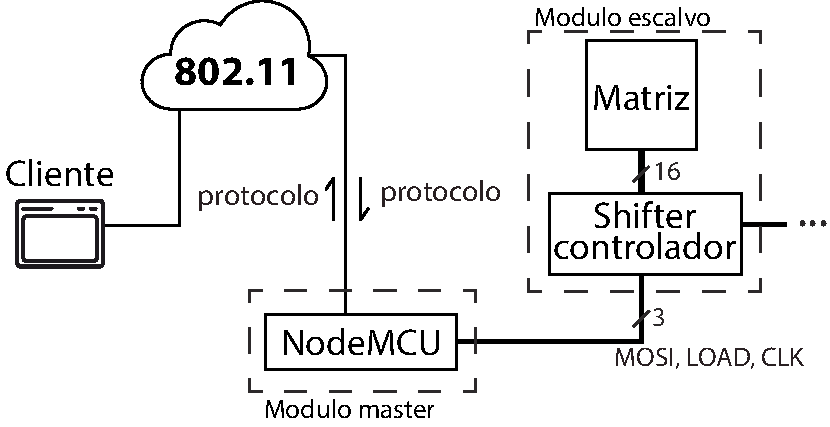
\includegraphics[width=\linewidth]{imagenes/hw/diagrama-bloques-general.pdf}
	\caption{Esquema general entre todos los componentes del sistema.}
	\label{fig:diagrama-bloques-general}
\end{figure}

\subsection{Fuente de alimentación}
\subsection{Módulo maestro}
\subsection{Módulo esclavo}
\subsection{Matriz de LEDs}
La matriz posee 64 LEDs organizados en ocho filas y ocho columnas, con cátodo común en las columnas como se observa en la \ref{fig:modulo-led}. Las medidas estan especificadas en la figura 

\begin{figure}[!ht]
	\centering
	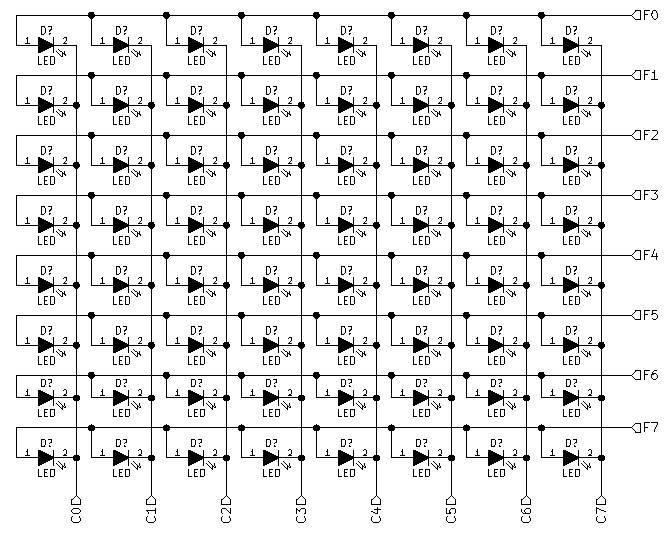
\includegraphics[width=0.7\linewidth]{imagenes/hw/modulo-led.pdf}
	\caption{Esquema de conexiones de la matriz de LEDs.}
	\label{fig:modulo-led}
\end{figure}
\begin{figure}[!ht]
	\centering
	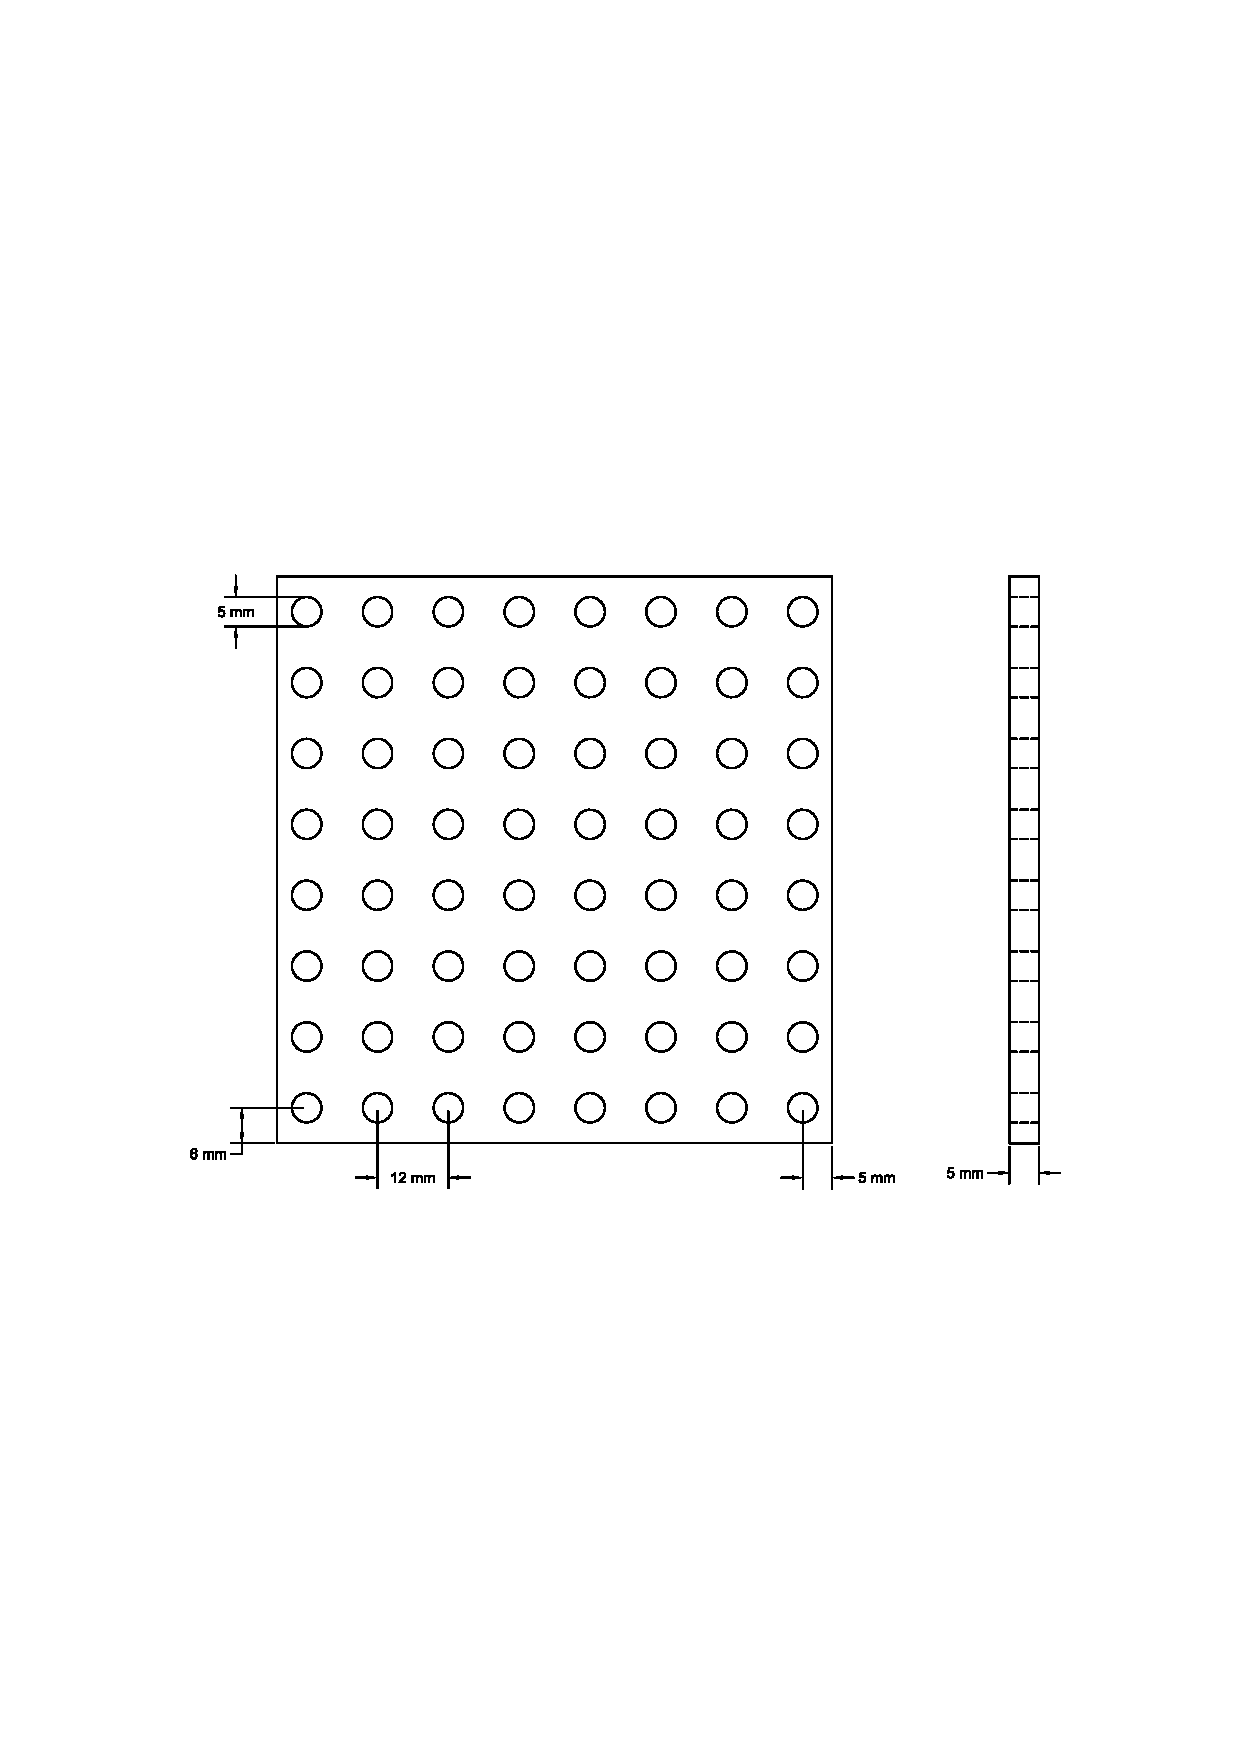
\includegraphics[width=0.7\linewidth]{imagenes/hw/modulo-led-dimensiones.pdf}
	\caption{Esquema de conexiones de la matriz de LEDs.}
	\label{fig:modulo-led-dimensiones}
\end{figure}


\subsection{Comunicación entre los módulos}

\section{Software}\label{sec:sw}
El software del sistema está formado por dos componentes: el firmware que corre sobre el controlador del cartel y la aplicación de PC que corre en una PC.

El cartel ser alcanzable por la PC a través de una red IP. Esto significa que no es estrictamente necesario que la PC y el cartel estén en una misma red física, sino que basta con que exista una ruta entre ellos. Sin embargo, el cartel está asociado a la red estrictamente mediante 802.11 (WiFi), mientras que la PC puede tener conectividad al cartel mediante diversas formas. Detalles básicos sobre el Internet Protocol y mecanismos de routeo no se discutirán en este informe.

\subsection{Interacción PC-Cartel}
La comunicación que se da entre la PC y el cartel sigue el modelo de Cliente-Servidor donde la PC es el cliente y el cartel es el servidor. Esto significa que es la PC quien comienza a interactuar con el cartel, estableciéndose un circuito virtual que permanecera activo cada vez que se quiera hacer un cambio de mensaje o configuración en el cartel, o incluso cuando se quiera recuperar el mensaje del cartel.

El tiempo que permanece activa la conexión debe ser, en lo posible, lo más corto posible. El cartel debe cerrar una conexión que permanezca ociosa por más de un tiempo configurable. La razón de esto es que un individuo malintencionado puede iniciar una conexión hacia el cartel y no mandar ningún mensaje, efectivamente bloqueando el uso legítimo del cartel (por limitaciones técnicas que se explicarán mas adelante, el controlador del cartel sólo puede aceptar una conexión a la vez). Se debe elegir un tiempo (a partir de ahora, tiempo de timeout) lo suficientemente corto para que esta medida sea efectiva pero no tan corto que descarte conexiones que legítimamente tienen un retardo (por ejemplo, por congestión de la red). Este tiempo es una constante ajustable en el código del firmware del cartel.

La figura \ref{fig:petri-net} describe el mecanismo de interacción entre la PC y el cartel mediante una red de Petri.

\begin{figure}[htbp]
	\centering
	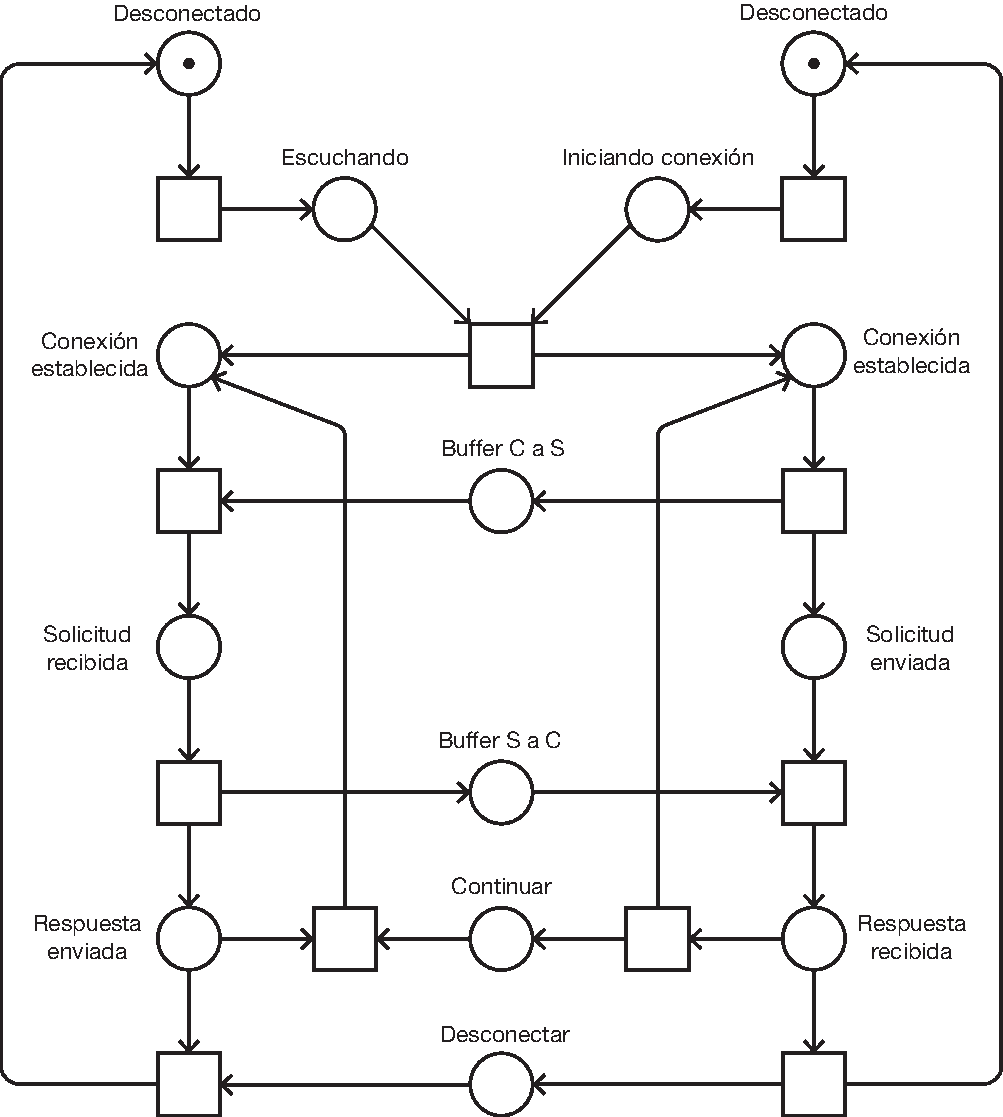
\includegraphics[width=\linewidth]{imagenes/petri-net.pdf}
	\caption{Red de Petri modelando la interacción entre la aplicación de PC y el cartel.}
	\label{fig:petri-net}
\end{figure}

\subsection{Firmware}
El firmware del controlador del cartel es quien se encarga de aceptar pedidos de la aplicación de PC y ejecutar las acciones de cambio de mensaje, parámetros de animacion, configuración WiFi o de contraseña. Además, como se explicó en la sección \ref{sec:hw}, el ESP8266EX envía la configuración de las matrices de LED por serie.

\subsection{Plataformas de desarrollo}
El System on Chip ESP8266EX es muy popular y existen diversas formas de desarrollar para él, entre ellas están:
\begin{itemize}
	\item El SDK oficial \enquote{OS} de Espressif. Es un SDK privativo. Utiliza internamente FreeRTOS con lo que se puede programar con tareas y las primitivas de sincronización que FreeRTOS ofrece.
	\item El SDK oficial \enquote{NON-OS} de Espressif. Tiene \enquote{NON-OS} en su nombre porque con este SDK el programador no puede especificar ni crear tareas propias. Sino que se limita a registrar funciones callbacks que son llamadas por el firmware de Espressif cuando suceden eventos. La programación termina siendo basada en eventos.
	\item La implementación de la plataforma Arduino para el ESP8266EX. Es la más sencilla de utilizar. Tiene las mismas abstracciones que se utilizan en la plataforma Arduino original. Incluye clases C++ que implementan servidores HTTP y hay mucho software y soporte disponible.
\end{itemize}

Todas estas formas de desarrollar tienen en común que el software del programador corre sobre un firmware privativo, es decir, no es viable programarlo \enquote{bare-metal} porque los registros y todos la información del hardware necesario para realizar algo no trivial no está disponible.

Para el este proyecto se decidió utilizar el SDK \enquote{NON-OS}, donde las funciones que define el programador se ejecutan siempre enteramente, de forma cooperativa. Esto elimina toda una clase de problemas de interferencia de datos a causa de la concurrencia, con lo que no es necesario utilizar primitivas de sincronización.
\subsubsection{Arquitectura del software}
\subsection{Aplicación de PC}
La aplicación de PC es un programa con interfaz gráfica que permite al usuario administrar el contenido y configuración del cartel de forma remota. En el marco del protocolo definido en el \ref{sec:protocolo}, la aplicación de PC es el cliente.

\subsubsection{Plataforma de desarrollo}
La aplicación está desarrollada en el \emph{framework} de desarrollo Qt. Qt es un conjunto muy amplio de librerías que permiten el desarrollo de aplicaciones gráficas que se pueden compilar para distintas plataformas (Windows, GNU/Linux, macOS o cualquier variante de Unix con X11). El lenguaje de programación que se utiliza es C++ con extensiones propias de Qt.

\subsubsection{Arquitectura basada en eventos}\label{sec:qt}
Qt permite desarrollar aplicaciones con una arquitectura basada en eventos. Sin embargo, la implementación de este sistema de eventos no está basada en los mecanismos más clásicos como el patrón Observer de la programación orientada a objetos ni el mecanismo de callbacks o punteros a funciones propios de la programación procedural, sino que hay métodos en los objetos que pueden ser denominados \emph{signals} o \emph{slots}.

Una clase puede tener opcionalmente uno o más métodos que sean \emph{signal} o \emph{slot}. La idea clave de estas sistema es que un objeto puede \enquote{emitir} una \emph{signal} que ejecuta el método \emph{slot} de otro objeto (o incluso posiblemente el mismo emisor) al cual se estableció previamente lo que se denomina \enquote{conexión}. Se ilustra este mecanismo en la figura \ref{fig:signals-slots}

\begin{figure}[!ht]
	\centering
	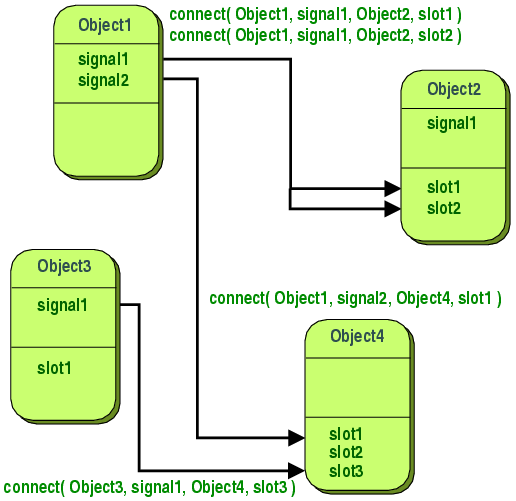
\includegraphics[height=8cm]{imagenes/signal-slots.png}
	\caption{Mecanismo de \emph{signal} y \emph{slot}.}
	\label{fig:signals-slots}
\end{figure}

En Qt, las clases que necesiten utilizar el sistema de eventos deben heredar de una clase provista por la librería llamada \code{QObject}. Esta clase provee distintas funcionalidades al resto de las clases definidas por Qt. Entre los objetos que heredan de QObject puede existir una relación de parentesco, en la cual un objeto $B$ puede tener como padre a otro objeto $A$. Esto, por ejemplo, sirve para liberar al programador del manejo de memoria: un objeto puede destruir a sus hijos antes de destruirse a sí mismo (por destrucción se entiende la liberación de todo recurso asociado al objeto, como memoria o archivos).

El mecanismo de \emph{signal} y \emph{slots} tiene como una de sus ventajas el hecho de que la ejecución de un \emph{slot} darse en otro hilo. Esto esta relacionado con la idea que promueve Qt de que un objeto puede "pertenecer" a un hilo de ejecución (encapsulado por la clase \code{QThread}), esto permite que no haya interferencia de datos causada por la concurrencia ya que no hay accesos explícitos a variables compartidas entre hilos sino que pueden enviar datos como argumentos a los \emph{slots}, de forma similar al paradigma de pasaje de mensajes en programación concurrentes.

Por ejemplo, en el caso del objeto \code{Object1} en la figura \ref{fig:signals-slots}, en algún método suyo se podría tener código como el siguiente:
\begin{lstlisting}[language=c++]
	// ...
	emit signal1();
	// ...
\end{lstlisting}

Mientras que \code{Object2} tiene un \emph{slot} llamado \code{slot1()} al cual \code{signal1()} de \code{Object1} está conectado. Entonces al emitirse \code{signal1()}, se ejecuta también \code{slot1} de \code{Object2} (además de los otros métodos pertenecientes a las otras clases que aparecen en la figura).

El momento en que se ejecuta un \emph{slot} depende del tipo de conexión que se haya establecido entre los objetos. Qt define tres tipos de conexiones:
\begin{description}
	\item[\code{DirectConnection}:] el \emph{slot} se ejecuta en el mismo hilo de ejecución desde el cual se hizo la emisión. Esto es útil para cuando los objetos que están conectados pertenecen a un mismo hilo o también cuando pertenecen a distintos hilos pero se toma precaución utilizando primitivas de sincronización para serializar el acceso al recurso o memoria compartida.
	\item[\code{QueuedConnection}:] se coloca un pedido de ejecución de \emph{slot} (con los argumentos que se hayan emitido) en la cola de eventos del hilo del objeto destino. Esto es lo que libera al programador de tener que utilizar primitivas de sincronización explícitas y es lo que se usa mayormente en la aplicación de PC de este proyecto. La ejecución de \code{emit} retorna inmediatamente, con lo que el hilo del objeto emisor no se bloquea al emitir una señal.
	\item[\code{BlockingQueuedConnection}:] Similar a \code{QueuedConnection}, con la diferencia que el hilo emisor se bloquea hasta que finalice la ejecución de los \emph{slots} que haya activado. Si no se utiliza con precaución y se establecen conexiones cíclicas, existe el riesgo de que ocurra un \emph{deadlock}, ocurrencia en la que un conjunto de hilos se espera entre sí indefinidamente, deteniendo parcial o íntegramente el programa.
\end{description}

Internamente, la implementación de Qt tiene una cola bloqueante de eventos para cada uno de los hilos que tengan una instancia de la clase \code{QThread}. También lleva registro de cuáles objetos que heredan de \code{QObject} pertenecen a cuál hilo. De esta manera, la ejecución de un hilo consiste principalmente en esperar a que hayan eventos para procesar en una cola bloqueante, cuya implementación específica depende de la plataforma para la cual se esté compilando el programa.

\subsubsection{Módulos}
En esta sección se listan las clases más relevantes de la aplicación de PC, sus métodos públicos principales y la interacción entre ellos.
Las clases son:
\begin{description}
	\item[\code{Panel}:] Provee la interfaz gráfica principal, que consiste en una ventana con los distintos elementos de control para que el usuario pueda manipular el cartel. Se puede ver una captura de pantalla en la figura \ref{fig:panel-screenshot}.
	\item[\code{Client}:] Realiza la interacción con el cartel a nivel mensaje del protocolo. Se encarga de generar los mensajes salientes y de tomar las acciones pertinentes ante una respuesta del cartel (servidor). La (única) instancia de esta clase \enquote{pertenece} (ver sección \ref{sec:qt}) a otro hilo en el cual se realizan todas las operaciones bloqueantes de entrada y salida, de forma que no se bloquea el hilo principal, que causaría que la interfaz gráfica deje de responder a eventos del sistema o del usuario.
	\item[\code{Connection}:] Abstrae la conexión al cartel, exponiendo métodos que envían y reciben específicamente los mensajes definidos en el protocolo. En esta clase también se hace la carga del certificado TLS antes de establecer una conexión.
	\item[\code{SignModel}:] Una clase \enquote{tonta} que agrupa todos los parámetros modificables del cartel, como el texto del cartel y sus parámetros de animación, los datos de la red Wifi a la que se debe conectar el cartel, etc. Existe principalmente para llevar registro de cuales parámetros fueron cambiados por el usuario y ameritan un pedido de cambio hacia el cartel. De manera que no se hagan cambios innecesarios al contenido o configuración del cartel.
\end{description}

\begin{figure}[!ht]
	\centering
	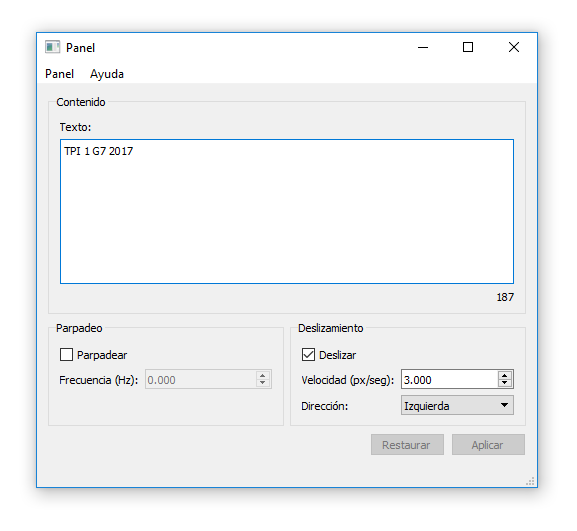
\includegraphics[height=10cm]{imagenes/panel-screenshot.png}
	\caption{captura de pantalla de la ventana principal de la aplicación de pc.}
	\label{fig:panel-screenshot}
\end{figure}

Se puede ver en la figura \ref{fig:uml-cliente} un diagrama de los objetos mencionados anteriormente. No están incluidas las conexiones entre los objetos para mantener la prolijidad del diagrama.

\begin{figure}[!ht]
	\centering
	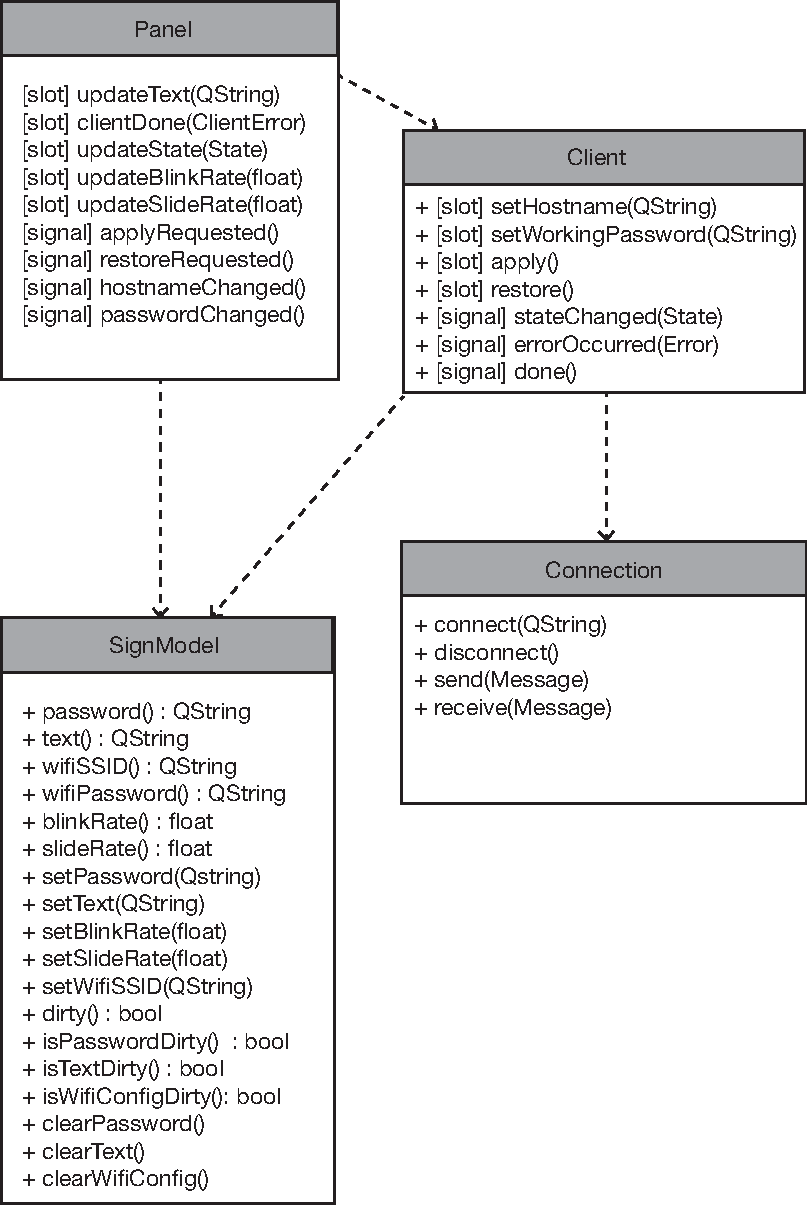
\includegraphics[scale=0.8]{imagenes/uml-cliente.pdf}
	\caption{Diagrama UML de las clases más relevantes.}
	\label{fig:uml-cliente}
\end{figure}

\subsection{Protocolo de comunicación}\label{sec:protocolo}
\subsubsection{Transport Layer Security}\label{sec:tls}


\clearpage
\part{Ensayos y mediciones}\label{part:ensayos}
\section{Conclusiones}
% Explicar el grado de cumplimiento de objetivos planteados para el trabajo.
% Evaluar y destacar el cumplimiento y disvíos del cronograma de tareas presentados en el informe inicial
% Describir claramente la actividad de cada integrante del grupo, evaluar las horas invertidas por cada uno y calcular las horas de ingeniería total
% Analizar el presupuesto que se ha invertido y el presupuesto final del proyecto incluyendo las horas de ingeniería consumidas.